%!TEX root = /Users/Ken/Work/Projects/LesHouches2017/STXSvsEFT/repo/LHStxsVsEft/Documentation/STXSvsSpecificEFTAna.tex
For the STXS sensitivity analysis, the generated samples for all signal benchmarks as well as the backgrounds (SM $pp \to ZH, H\to b\bar{b}$ and $pp\to Zb\bar{b}$) are categorized according to the STXS proposal for the $VH$ channel in Ref.~\cite{deFlorian:2016spz}. Within this framework, different regions of the phase space --referred to as ``bins'' for simplicity-- are defined, with the purpose of optimizing the sensitivity of the measurements while at the same time minimizing their dependence on theory assumptions. The different STXS bins are defined specifically for each Higgs production mode. For our process of interest ($pp \to ZH \to \ell^+ \ell^- b\bar{b}$) the different stages of the categorization and the resulting bins are summarized as follows (see \cite{deFlorian:2016spz} for details):
\vspace{0.5cm}
%
\begin{itemize}
{\item  {\bf Stage 0:} Events with $\left|y_H\right| <2.5$ are selected.}
%
{\item {\bf Stage 1:} $ZH$ production is split into $q\bar{q}$ and $gg$ initial states (our process sample was generated at LO and therefore only contains $q\bar{q}\to ZH$ events). Events are subsequently classified according to the value of $p_T^Z$ and number of extra jets in the event as follows:
%
\vspace{0.25cm}
%
\begin{center}
${\bf \underline{q\bar{q}\to ZH}}$
\end{center}
\begin{eqnarray}
p_T^Z \in& [0,150]~\mathrm{GeV},& \nonumber\\
%
p_T^Z \in& [150,250]~\mathrm{GeV}&(0\mbox{-}\mathrm{j}),\\
%
p_T^Z \in& [150,250]~\mathrm{GeV}&(\geq 1\mbox{-}\mathrm{j}),\nonumber\\
%
p_T^Z >&250~\mathrm{GeV}.\nonumber&
\end{eqnarray}
}
%
%
{\item {\bf Stage 2:} On this last stage the low $p_T^Z$ bins are further separated according to the number of extra jets, while the high-$p_T^Z$ region is split at 400 GeV. The final set of STXS bins that apply in our case are the following six:
%
\vspace{0.25cm}
%
\begin{center}
${\bf \underline{q\bar{q}\to ZH}}$
\end{center}
\begin{eqnarray}
p_T^Z \in& [0,150]~\mathrm{GeV}&(0\mbox{-}\mathrm{j}),\nonumber\\
%
p_T^Z \in& [0,150]~\mathrm{GeV}&(\geq 1\mbox{-}\mathrm{j}),\nonumber\nonumber\\
%
p_T^Z \in& [150,250]~\mathrm{GeV}&(0\mbox{-}\mathrm{j}),\\
%
p_T^Z \in& [150,250]~\mathrm{GeV}&(\geq 1\mbox{-}\mathrm{j}),\nonumber\\
%
p_T^Z \in& [250,400]~\mathrm{GeV},&\nonumber\\
%
p_T^Z >&400~\mathrm{GeV}.\nonumber&
\end{eqnarray}
}
\end{itemize}
%
In order to profit from the maximum amount of available information, we use the stage 2 categorisation to compare with the multivariate analysis. Additionally, we use the BDT discriminant, $p(Z b\bar{b})$, trained to reject the $Zb\bar{b}$ background in favour of SM $ZH$, described in Section~\ref{sec:training} to purify our event sample. Our STXS yields are computed after cutting on this discriminant with 18.6\% efficiency for SM $ZH$  and $> 99\%$ rejection for $Zb\bar{b}$. No extra information or discriminant to enhance sensitivity to new physics is used, consistently with the STXS hypotheses.  Figure~\ref{fig:stxs_crosssec} shows the predicted cross sections for the various samples in the STXS bins. The $Zb\bar{b}$ contribution has clearly been brought under control by the BDT discriminant. In the bins that have been split by jet multiplicity, this contribution appears to have a larger relative increase when going from zero to one or more jets, probably owing to the dominant $gg$-initiated contribution to this process increasing the radiation probability. We see that the EFT contributions diverge from the SM prediction with increasing $p_T$, as expected, and the $Zb\bar{b}$ background also becomes less and less important. 

\begin{figure}[h!]
\centering
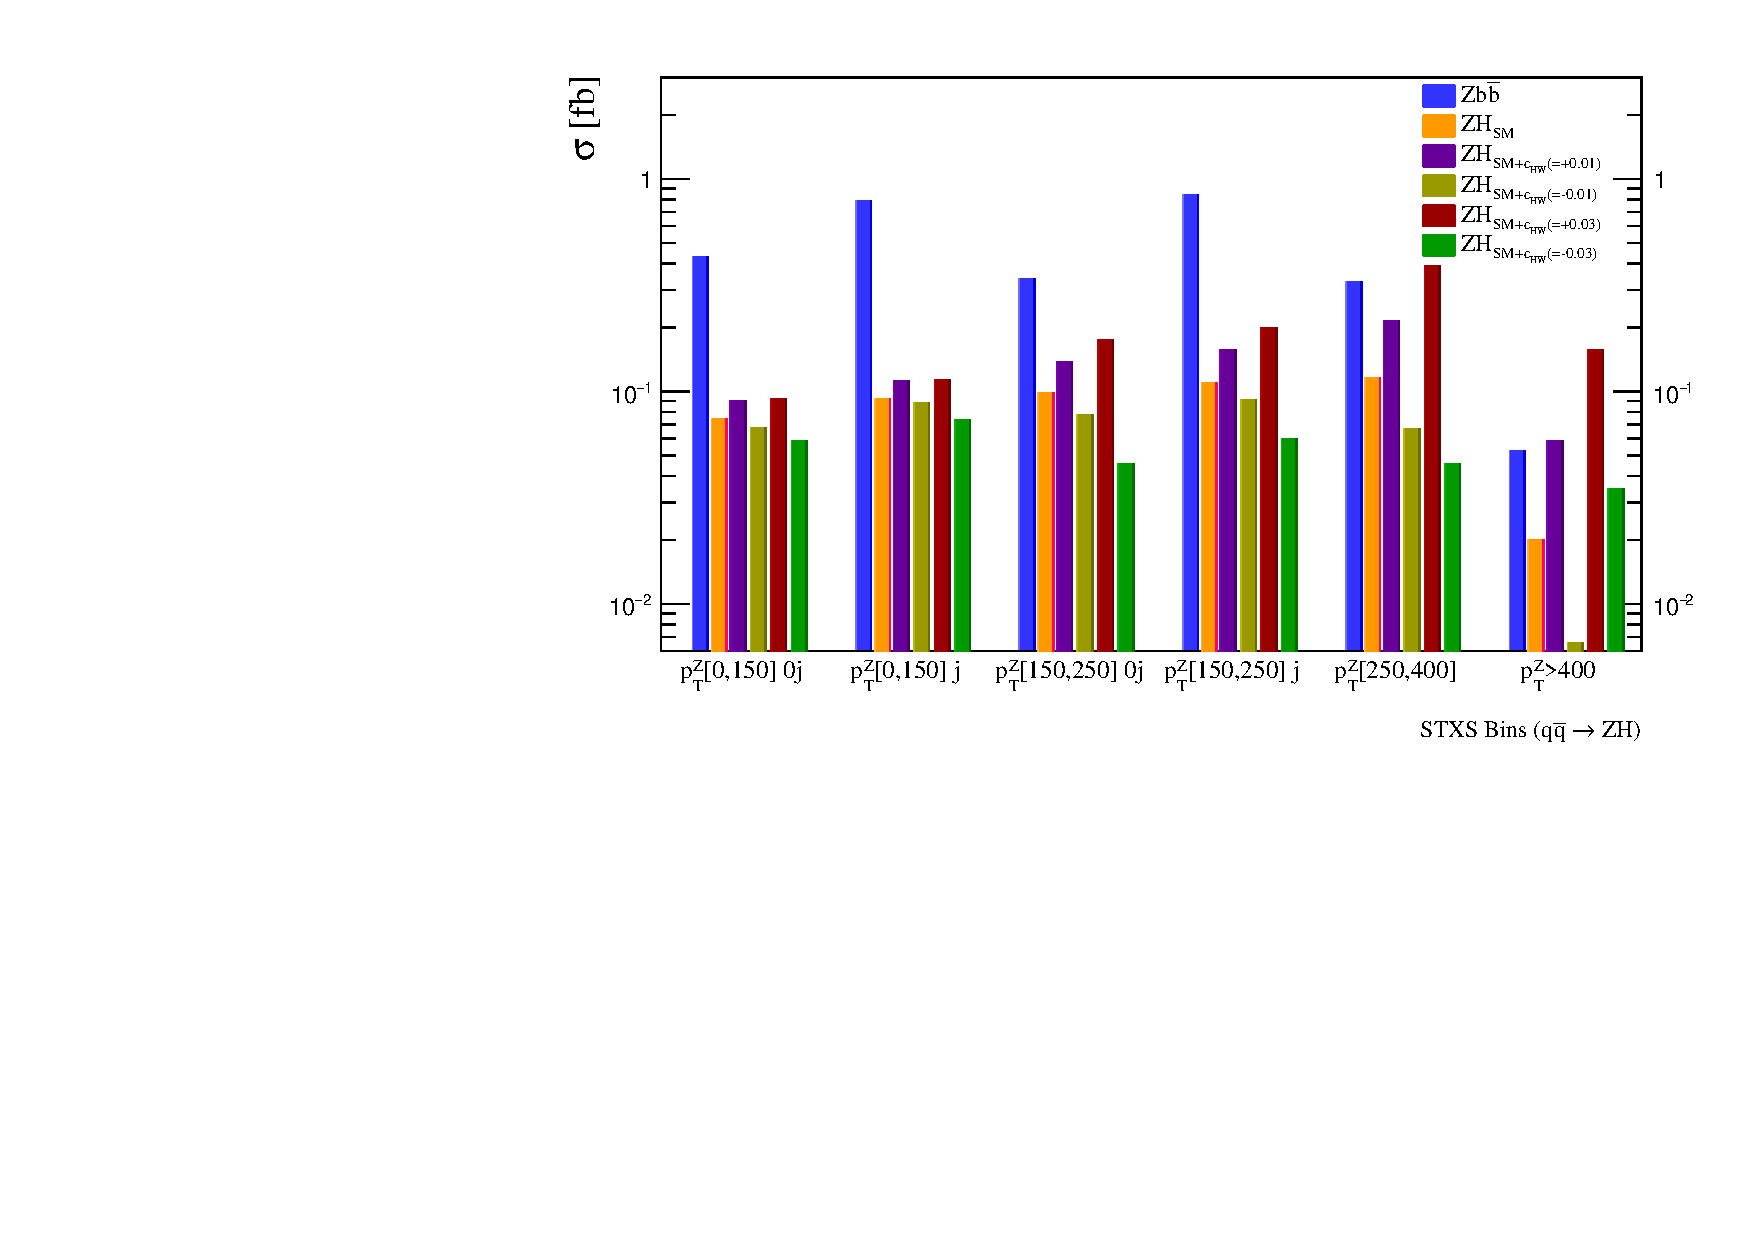
\includegraphics[width=0.6\textwidth]{plots/STXS_comp.pdf}
\caption{
\label{fig:stxs_crosssec}
Predicted cross sections in the stage 2, $ZH$ STXS bins for SM $ZH$ production as well as our four EFT benchmarks and the $Zb\bar{b}$ background. The cross sections correspond to events passing the basic fiducial selection of Section~\ref{sec:fiducial}, accounting for $b$-tagging efficiencies and after applying a cut on the $Zb\bar{b}$ BDT discriminant as described in the text.
    }
\end{figure}






